\documentclass[a4paper,12pt,twoside,onecolumn,openright,final,oldfontcommands]{memoir}
\usepackage{lmodern}
\usepackage{amssymb,amsmath}
\usepackage{ifxetex,ifluatex}
\usepackage{fixltx2e} % provides \textsubscript
\ifnum 0\ifxetex 1\fi\ifluatex 1\fi=0 % if pdftex
  \usepackage[T1]{fontenc}
  \usepackage[utf8]{inputenc}
\else % if luatex or xelatex
  \ifxetex
    \usepackage{mathspec}
  \else
    \usepackage{fontspec}
  \fi
  \defaultfontfeatures{Ligatures=TeX,Scale=MatchLowercase}
\fi
% use upquote if available, for straight quotes in verbatim environments
\IfFileExists{upquote.sty}{\usepackage{upquote}}{}
% use microtype if available
\IfFileExists{microtype.sty}{%
\usepackage{microtype}
\UseMicrotypeSet[protrusion]{basicmath} % disable protrusion for tt fonts
}{}
\usepackage[unicode=true]{hyperref}
\hypersetup{
            pdftitle={From mechanistic modelling of cancer to clinical interpretation and impact evaluation},
            pdfborder={0 0 0},
            breaklinks=true}
\urlstyle{same}  % don't use monospace font for urls
\usepackage{natbib}
\bibliographystyle{plainnat}
\usepackage{color}
\usepackage{fancyvrb}
\newcommand{\VerbBar}{|}
\newcommand{\VERB}{\Verb[commandchars=\\\{\}]}
\DefineVerbatimEnvironment{Highlighting}{Verbatim}{commandchars=\\\{\}}
% Add ',fontsize=\small' for more characters per line
\usepackage{framed}
\definecolor{shadecolor}{RGB}{248,248,248}
\newenvironment{Shaded}{\begin{snugshade}}{\end{snugshade}}
\newcommand{\KeywordTok}[1]{\textcolor[rgb]{0.13,0.29,0.53}{\textbf{{#1}}}}
\newcommand{\DataTypeTok}[1]{\textcolor[rgb]{0.13,0.29,0.53}{{#1}}}
\newcommand{\DecValTok}[1]{\textcolor[rgb]{0.00,0.00,0.81}{{#1}}}
\newcommand{\BaseNTok}[1]{\textcolor[rgb]{0.00,0.00,0.81}{{#1}}}
\newcommand{\FloatTok}[1]{\textcolor[rgb]{0.00,0.00,0.81}{{#1}}}
\newcommand{\ConstantTok}[1]{\textcolor[rgb]{0.00,0.00,0.00}{{#1}}}
\newcommand{\CharTok}[1]{\textcolor[rgb]{0.31,0.60,0.02}{{#1}}}
\newcommand{\SpecialCharTok}[1]{\textcolor[rgb]{0.00,0.00,0.00}{{#1}}}
\newcommand{\StringTok}[1]{\textcolor[rgb]{0.31,0.60,0.02}{{#1}}}
\newcommand{\VerbatimStringTok}[1]{\textcolor[rgb]{0.31,0.60,0.02}{{#1}}}
\newcommand{\SpecialStringTok}[1]{\textcolor[rgb]{0.31,0.60,0.02}{{#1}}}
\newcommand{\ImportTok}[1]{{#1}}
\newcommand{\CommentTok}[1]{\textcolor[rgb]{0.56,0.35,0.01}{\textit{{#1}}}}
\newcommand{\DocumentationTok}[1]{\textcolor[rgb]{0.56,0.35,0.01}{\textbf{\textit{{#1}}}}}
\newcommand{\AnnotationTok}[1]{\textcolor[rgb]{0.56,0.35,0.01}{\textbf{\textit{{#1}}}}}
\newcommand{\CommentVarTok}[1]{\textcolor[rgb]{0.56,0.35,0.01}{\textbf{\textit{{#1}}}}}
\newcommand{\OtherTok}[1]{\textcolor[rgb]{0.56,0.35,0.01}{{#1}}}
\newcommand{\FunctionTok}[1]{\textcolor[rgb]{0.00,0.00,0.00}{{#1}}}
\newcommand{\VariableTok}[1]{\textcolor[rgb]{0.00,0.00,0.00}{{#1}}}
\newcommand{\ControlFlowTok}[1]{\textcolor[rgb]{0.13,0.29,0.53}{\textbf{{#1}}}}
\newcommand{\OperatorTok}[1]{\textcolor[rgb]{0.81,0.36,0.00}{\textbf{{#1}}}}
\newcommand{\BuiltInTok}[1]{{#1}}
\newcommand{\ExtensionTok}[1]{{#1}}
\newcommand{\PreprocessorTok}[1]{\textcolor[rgb]{0.56,0.35,0.01}{\textit{{#1}}}}
\newcommand{\AttributeTok}[1]{\textcolor[rgb]{0.77,0.63,0.00}{{#1}}}
\newcommand{\RegionMarkerTok}[1]{{#1}}
\newcommand{\InformationTok}[1]{\textcolor[rgb]{0.56,0.35,0.01}{\textbf{\textit{{#1}}}}}
\newcommand{\WarningTok}[1]{\textcolor[rgb]{0.56,0.35,0.01}{\textbf{\textit{{#1}}}}}
\newcommand{\AlertTok}[1]{\textcolor[rgb]{0.94,0.16,0.16}{{#1}}}
\newcommand{\ErrorTok}[1]{\textcolor[rgb]{0.64,0.00,0.00}{\textbf{{#1}}}}
\newcommand{\NormalTok}[1]{{#1}}
\usepackage{longtable,booktabs}
\usepackage{graphicx,grffile}
\makeatletter
\def\maxwidth{\ifdim\Gin@nat@width>\linewidth\linewidth\else\Gin@nat@width\fi}
\def\maxheight{\ifdim\Gin@nat@height>\textheight\textheight\else\Gin@nat@height\fi}
\makeatother
% Scale images if necessary, so that they will not overflow the page
% margins by default, and it is still possible to overwrite the defaults
% using explicit options in \includegraphics[width, height, ...]{}
\setkeys{Gin}{width=\maxwidth,height=\maxheight,keepaspectratio}
\IfFileExists{parskip.sty}{%
\usepackage{parskip}
}{% else
\setlength{\parindent}{0pt}
\setlength{\parskip}{6pt plus 2pt minus 1pt}
}
\setlength{\emergencystretch}{3em}  % prevent overfull lines
\providecommand{\tightlist}{%
  \setlength{\itemsep}{0pt}\setlength{\parskip}{0pt}}
\setcounter{secnumdepth}{5}
% Redefines (sub)paragraphs to behave more like sections
\ifx\paragraph\undefined\else
\let\oldparagraph\paragraph
\renewcommand{\paragraph}[1]{\oldparagraph{#1}\mbox{}}
\fi
\ifx\subparagraph\undefined\else
\let\oldsubparagraph\subparagraph
\renewcommand{\subparagraph}[1]{\oldsubparagraph{#1}\mbox{}}
\fi
%%%%%%%%%%%%%%%%%%%%%%%%%%%%%%%%%%%%%%%%%%%%%%%%%%%%%%%%%%%%%
%Start preamble
%%%%%%%%%%%%%%%%%%%%%%%%%%%%%%%%%%%%%%%%%%%%%%%%%%%%%%%%%%%%%

\usepackage{booktabs}
\usepackage{amsthm}
\usepackage{./cover/psl-cover} % specifies the path to the cover page template

%\makeatletter
%\def\thm@space@setup{%
%  \thm@preskip=8pt plus 2pt minus 4pt
%  \thm@postskip=\thm@preskip
%}
%\makeatother


%%%%%%%%%%%%%%%%%%%%%%%%%%%%%%%%%%%%%%%%%%%%%%%%%%%%%%%%%%%%%
% Add a lettrine to the very first character of the content %
%%%%%%%%%%%%%%%%%%%%%%%%%%%%%%%%%%%%%%%%%%%%%%%%%%%%%%%%%%%%%

\usepackage{lettrine} % supports various dropped capitals styles

\newcommand{\initial}[1]{
	\lettrine[lines=3,lhang=0.33,nindent=0em]{
		\color{gray}
     		{\textsc{#1}}}{}}
     		
%%%%%%%%%%%%%%%%%%%%%%%%
% Insert an empty page %
%%%%%%%%%%%%%%%%%%%%%%%%

\usepackage{afterpage} % executes command after the next page break

\newcommand\blankpage{%
    \null
    \thispagestyle{empty}%
    % \addtocounter{page}{-1}% % uncomment to increase page counter
    \newpage
    }

\newcommand{\clearemptydoublepage}{\newpage{\thispagestyle{empty}\cleardoublepage}}

%%%%%%%%%%%%%%%%%%
% Epigraph style %
%%%%%%%%%%%%%%%%%%

\usepackage{epigraph} % provides commands to assist in the typesetting of a single epigraph

\setlength\epigraphwidth{1\textwidth}
\setlength\epigraphrule{0pt} % no line between
\setlength\beforeepigraphskip{1\baselineskip} % space before and after epigraph
\setlength\afterepigraphskip{2\baselineskip}
\renewcommand*{\textflush}{flushright}
\renewcommand*{\epigraphsize}{\normalsize\itshape}

%%%%%%%%%%%%%%%%%%%%%%%%
% Formatting
%%%%%%%%%%%%%%%%%%%%

\usepackage{calc} % simple arithmetics in latex commands
\usepackage{soul} % hyphenation for letterspacing, underlining, etc.

\makeatletter
\newlength\dlf@normtxtw
\setlength\dlf@normtxtw{\textwidth}
\newsavebox{\feline@chapter}
\newcommand\feline@chapter@marker[1][4cm]{%
	\sbox\feline@chapter{%
		\resizebox{!}{#1}{\fboxsep=1pt%
			\colorbox{gray}{\color{white}\thechapter}%
		}}%
		\rotatebox{90}{%
			\resizebox{%
				\heightof{\usebox{\feline@chapter}}+\depthof{\usebox{\feline@chapter}}}%
			{!}{\scshape\so\@chapapp}}\quad%
		\raisebox{\depthof{\usebox{\feline@chapter}}}{\usebox{\feline@chapter}}%
}

\newcommand\feline@chm[1][4cm]{%
	\sbox\feline@chapter{\feline@chapter@marker[#1]}%
	\makebox[0pt][c]{% aka \rlap
		\makebox[1cm][r]{\usebox\feline@chapter}%
	}}

\makechapterstyle{daleifmodif}{
\renewcommand\chapnamefont{\normalfont\Large\scshape\raggedleft\so}
\renewcommand\chaptitlefont{\normalfont\Large\bfseries\scshape}
\renewcommand\chapternamenum{} \renewcommand\printchaptername{}
\renewcommand\printchapternum{\null\hfill\feline@chm[2.5cm]\par}
\renewcommand\afterchapternum{\par\vskip\midchapskip}
\renewcommand\printchaptertitle[1]{\color{gray}\chaptitlefont\raggedleft
  \renewcommand\chaptername{Chapter}
  ##1\par}
}

\makeatother
\chapterstyle{daleifmodif}

% The pages should be numbered consecutively at the bottom centre of the page
\makepagestyle{myvf}
\makeoddfoot{myvf}{}{\thepage}{}
\makeevenfoot{myvf}{}{\thepage}{}
\makeheadrule{myvf}{\textwidth}{\normalrulethickness}
\makeevenhead{myvf}{\small\textsc{\leftmark}}{}{}
\makeoddhead{myvf}{}{}{\small\textsc{\rightmark}}
\pagestyle{myvf}


%%%%%%%%%%%%%%%%%%%%%%%%%%%%%%%%%%%%%%%%%%%%%%%%%%%%%%%%%%%%%
% Define cover page settings
%%%%%%%%%%%%%%%%%%%%%%%%%%%%%%%%%%%%%%%%%%%%%%%%%%%%%%%%%%%%%

\title{My title}

\author{Jonas BEAL}

\institute{l'Institut Curie}
\doctoralschool{Complexite du Vivant}{515}

\institute{l'Institut Curie}
\doctoralschool{Complexité du Vivant}{515}
\specialty{Génomique}
\date{15 septembre 2020}

%% cotutelle
% \entitle{Thesis Subject in English}
% \otherinstitute{CEA Saclay}
% \logootherinstitute{logo-institute}

\jurymember{1}{Test NOM}{Titre, Établissement}{Président}
\jurymember{2}{Test NOM}{Titre, Établissement}{Rapporteur}
\jurymember{3}{Test NOM}{Titre, Établissement}{Examinateur}
\jurymember{4}{Test NOM}{Titre, Établissement}{Examinateur}
\jurymember{5}{Emmanuel BARILLOT}{Institut Curie, INSERM, Mines ParisTech, PSL}{Directeur de thèse}
\jurymember{6}{Aurélien LATOUCHE}{Institut Curie, Cnam}{Directeur de thèse}
\jurymember{7}{Laurence CALZONE}{Institut Curie, INSERM, Mines ParisTech, PSL}{Co-encadrante de thèse}
% \jurymember{9}{Prénom NOM}{Titre, établissement}{Invité}
% \jurymember{10}{Prénom NOM}{Titre, établissement}{Invité}

\frabstract{
  Cuius acerbitati uxor grave accesserat incentivum,
  germanitate Augusti turgida supra modum, quam Hannibaliano
  regi fratris filio antehac Constantinus iunxerat pater,
  Megaera quaedam mortalis, inflammatrix saevientis adsidua,
  humani cruoris avida nihil mitius quam maritus; qui paulatim
  eruditiores facti processu temporis ad nocendum per
  clandestinos versutosque rumigerulos conpertis leviter
  addere quaedam male suetos falsa et placentia sibi
  discentes, adfectati regni vel artium nefandarum calumnias
  insontibus adfligebant.

}

\enabstract{
  Verum ad istam omnem orationem brevis est defensio. Nam
  quoad aetas M. Caeli dare potuit isti suspicioni locum, fuit
  primum ipsius pudore, deinde etiam patris diligentia
  disciplinaque munita. Qui ut huic virilem togam dedit nihil
  dicam hoc loco de me; tantum sit, quantum vos existimatis;
  hoc dicam, hunc a patre continuo ad me esse deductum; nemo
  hunc M. Caelium in illo aetatis flore vidit nisi aut cum
  patre aut mecum aut in M. Crassi castissima domo, cum
  artibus honestissimis erudiretur.

}

\frkeywords{ Caesar licentia post honoratis haec adhibens urbium
  honoratis nullum Caesar.}
\enkeywords{ Delatus delatus nominatus
  onere aut trahebatur quod tenus et bonorum.}
  
\pagenumbering{roman}

\title{From mechanistic modelling of cancer to clinical interpretation and
impact evaluation}
\date{15/09/2020}

\begin{document}
\maketitle

\chapter*{Abstract}

\initial{L}orem ipsum dolor sit amet, consectetur adipiscing elit, sed
do eiusmod tempor incididunt ut labore et dolore magna aliqua. Ut enim
ad minim veniam, quis nostrud exercitation ullamco laboris nisi ut
aliquip ex ea commodo consequat.

Duis aute irure dolor in reprehenderit in voluptate velit esse cillum
dolore eu fugiat nulla pariatur. Excepteur sint occaecat cupidatat non
proident, sunt in culpa qui officia deserunt mollit anim id est laborum

\vspace{\baselineskip}

\textbf{Key-words}:

\chapter*{Résumé}

\initial{L}orem ipsum dolor sit amet, consectetur adipiscing elit, sed
do eiusmod tempor incididunt ut labore et dolore magna aliqua. Ut enim
ad minim veniam, quis nostrud exercitation ullamco laboris nisi ut
aliquip ex ea commodo consequat. Duis aute irure dolor in reprehenderit
in voluptate velit esse cillum dolore eu fugiat nulla pariatur.

Excepteur sint occaecat cupidatat non proident, sunt in culpa qui
officia deserunt mollit anim id est laborum

\vspace{\baselineskip}

\textbf{Mots-clés}:

\afterpage{\blankpage}

\chapter*{Acknowledgements}

\initial{M}any persons to thanks. Lorem ipsum dolor sit amet,
consectetur adipiscing elit, sed do eiusmod tempor incididunt ut labore
et dolore magna aliqua. Ut enim ad minim veniam, quis nostrud
exercitation ullamco laboris nisi ut aliquip ex ea commodo consequat.

Duis aute irure dolor in reprehenderit in voluptate velit esse cillum
dolore eu fugiat nulla pariatur. Excepteur sint occaecat cupidatat non
proident, sunt in culpa qui officia deserunt mollit anim id est laborum

\clearemptydoublepage

\renewcommand{\contentsname}{Table of contents}

\maxtocdepth{subsection}

\tableofcontents*
\addtocontents{toc}{\par\nobreak \mbox{}\hfill{\bf Page}\par\nobreak}
\newpage

\listoftables
\addtocontents{lot}{\par\nobreak\textbf{{\scshape Table} \hfill Page}\par\nobreak}
\newpage

\listoffigures
\addtocontents{lof}{\par\nobreak\textbf{{\scshape Figure} \hfill Page}\par\nobreak}
\newpage

\blankpage

\pagenumbering{arabic}

\part{Cells and their
models}\label{part-cells-and-their-models}

\chapter{Scientific modeling: abstract the
complexity}\label{scientific-modeling-abstract-the-complexity}

\epigraph{"Ce qui est simple est toujours faux. Ce qui ne l'est pas est inutilisable."}{Paul Valéry (Mauvaises pensées et autres, 1942)}

\initial{T}he notion of modeling is embedded in science, to the point
that it has sometimes been used to define the very nature of scientific
research. What is called a model can, however, correspond to very
different realities which need to be defined before addressing the
object of this thesis which will consist, if one wants to be
mischievous, in analyzing models with other models. This semantic
elucidation is all the more necessary as this thesis is
interdisciplinary, suspended between systems biology and biostatistics.
In order to convince the reader of the need for such a preamble, he is
invited to ask a statistician and a systems biologist the question how
they would define what a model is.

\begin{figure}

{\centering \includegraphics[width=0.9\linewidth]{fig/orrery} 

}

\caption[A scientist and his model]{\textbf{A scientist and his model.} Joseph Wright
of Derby, \emph{A Philosopher Giving a Lecture at the Orrery (in which a
lamp is put in place of the sun)}, c. 1763-65, oil on canvas, Derby
Museums and Art Gallery}\label{fig:orrery}
\end{figure}






\section{What is a model?}\label{what-is-a-model}

A model is first of all an ambiguous object and a polysemous word.Among
the many meanings proposed by the dictionary \ref{fig:visualThesaurus},
several even find echoes in scientific practice. It is sometimes a
question of the physical representation of an object, often on a reduced
scale, and sometimes of a theoretical description intended to facilitate
the understanding of the way in which a system works, or even sometimes
an ideal to achieve \citep{dictionnarymodel}.

\begin{figure}

{\centering 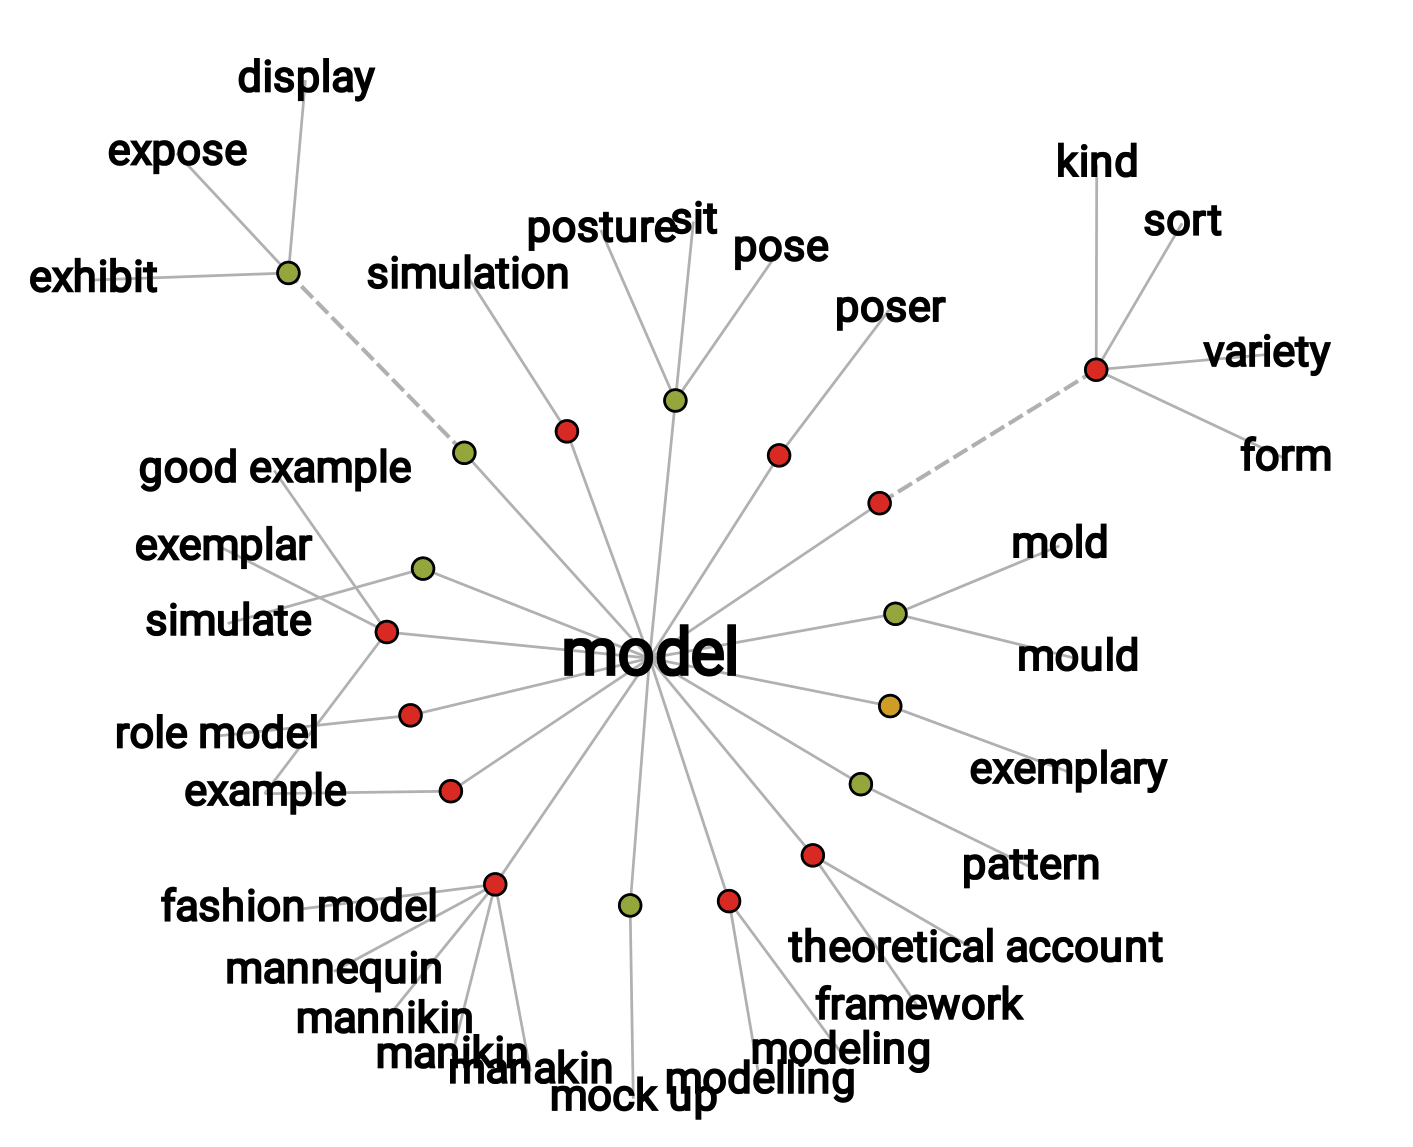
\includegraphics[width=0.9\linewidth]{fig/visualThesaurus} 

}

\caption[Network visualization of *model* thesaurus entries]{\textbf{Network visualization of
\emph{model} thesaurus entries.} Generated with the
\href{https://www.visualthesaurus.com}{`Visual Thesaurus'} ressource}\label{fig:visual-thesaurus}
\end{figure}





Different conceptions between scientists but common patterns
\citep{bailer2002scientists}: models provide insights about the topic
under investigation, often at a cost of simplification. Not required to
be right but should be valid (depends on the objective). May be able to
predict or at least to test.

Pubmed tree

Material/physical models (from orrery to drosophila) Formal/theoretical
models

``No substantial part of the universe is so simple that it can be
grasped and controlled without abstraction. Abstraction consists in
replacing the part of the universe under consideration by a model of
similar but simpler structure. Models, formal and intellectual on the
one hand, or material on the other, are thus a central necessity of
scientific procedure.''
\url{https://www.nemenmanlab.org/~ilya/images/9/99/Rosenblueth-wiener-1945.pdf}

Philosophy \citep{frigg2006models}

Galilean idealization with reality distortion But even toy models for
salient features

Historically physical models

Then mathematics as a language

Statistical models with a priori knowledge

In vivo, in vitro, in silico,

\section{Statistical modeling}\label{statistical-modeling}

Within formal models -\textgreater{} 2 kinds

\citep{baker2018mechanistic}

\url{https://gosilico.com/technology/mechanistic-vs-statistical-models/}

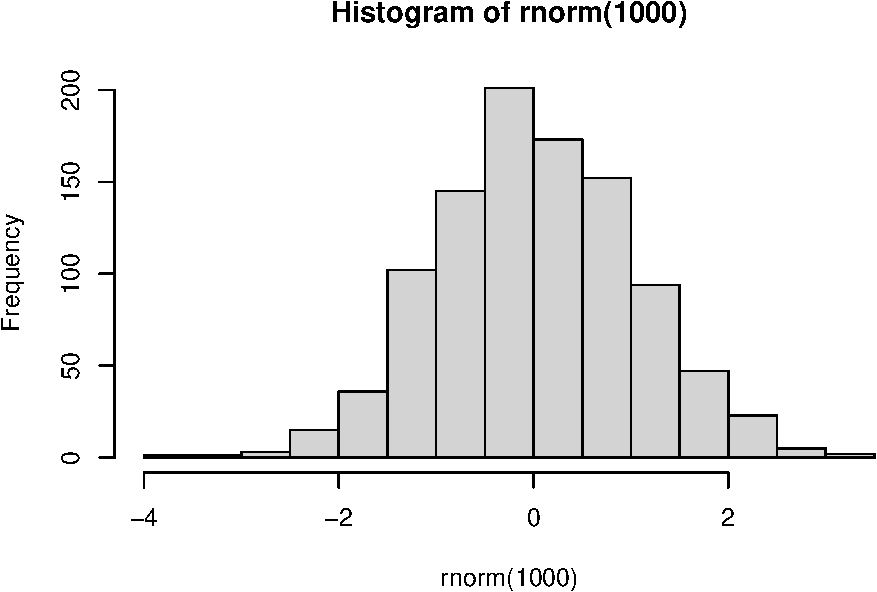
\includegraphics{01-Models_files/figure-latex/figure_ext-1.pdf}

\section{Mechanistic modeling}\label{mechanistic-modeling}

\chapter{What is cancer}\label{what-is-cancer}

This is a test

\section{Abc}\label{abc}

Bla bla

The LaTeX environment \texttt{tiny} is only generated for LaTeX output.

\begin{tiny}


\begin{tabular}{l|r|r|r|r|r|r|r|r|r|r|r}
\hline
  & mpg & cyl & disp & hp & drat & wt & qsec & vs & am & gear & carb\\
\hline
Mazda RX4 & 21.0 & 6 & 160.0 & 110 & 3.90 & 2.620 & 16.46 & 0 & 1 & 4 & 4\\
\hline
Mazda RX4 Wag & 21.0 & 6 & 160.0 & 110 & 3.90 & 2.875 & 17.02 & 0 & 1 & 4 & 4\\
\hline
Datsun 710 & 22.8 & 4 & 108.0 & 93 & 3.85 & 2.320 & 18.61 & 1 & 1 & 4 & 1\\
\hline
Hornet 4 Drive & 21.4 & 6 & 258.0 & 110 & 3.08 & 3.215 & 19.44 & 1 & 0 & 3 & 1\\
\hline
Hornet Sportabout & 18.7 & 8 & 360.0 & 175 & 3.15 & 3.440 & 17.02 & 0 & 0 & 3 & 2\\
\hline
Valiant & 18.1 & 6 & 225.0 & 105 & 2.76 & 3.460 & 20.22 & 1 & 0 & 3 & 1\\
\hline
Duster 360 & 14.3 & 8 & 360.0 & 245 & 3.21 & 3.570 & 15.84 & 0 & 0 & 3 & 4\\
\hline
Merc 240D & 24.4 & 4 & 146.7 & 62 & 3.69 & 3.190 & 20.00 & 1 & 0 & 4 & 2\\
\hline
Merc 230 & 22.8 & 4 & 140.8 & 95 & 3.92 & 3.150 & 22.90 & 1 & 0 & 4 & 2\\
\hline
Merc 280 & 19.2 & 6 & 167.6 & 123 & 3.92 & 3.440 & 18.30 & 1 & 0 & 4 & 4\\
\hline
Merc 280C & 17.8 & 6 & 167.6 & 123 & 3.92 & 3.440 & 18.90 & 1 & 0 & 4 & 4\\
\hline
Merc 450SE & 16.4 & 8 & 275.8 & 180 & 3.07 & 4.070 & 17.40 & 0 & 0 & 3 & 3\\
\hline
Merc 450SL & 17.3 & 8 & 275.8 & 180 & 3.07 & 3.730 & 17.60 & 0 & 0 & 3 & 3\\
\hline
Merc 450SLC & 15.2 & 8 & 275.8 & 180 & 3.07 & 3.780 & 18.00 & 0 & 0 & 3 & 3\\
\hline
Cadillac Fleetwood & 10.4 & 8 & 472.0 & 205 & 2.93 & 5.250 & 17.98 & 0 & 0 & 3 & 4\\
\hline
Lincoln Continental & 10.4 & 8 & 460.0 & 215 & 3.00 & 5.424 & 17.82 & 0 & 0 & 3 & 4\\
\hline
Chrysler Imperial & 14.7 & 8 & 440.0 & 230 & 3.23 & 5.345 & 17.42 & 0 & 0 & 3 & 4\\
\hline
Fiat 128 & 32.4 & 4 & 78.7 & 66 & 4.08 & 2.200 & 19.47 & 1 & 1 & 4 & 1\\
\hline
Honda Civic & 30.4 & 4 & 75.7 & 52 & 4.93 & 1.615 & 18.52 & 1 & 1 & 4 & 2\\
\hline
Toyota Corolla & 33.9 & 4 & 71.1 & 65 & 4.22 & 1.835 & 19.90 & 1 & 1 & 4 & 1\\
\hline
Toyota Corona & 21.5 & 4 & 120.1 & 97 & 3.70 & 2.465 & 20.01 & 1 & 0 & 3 & 1\\
\hline
Dodge Challenger & 15.5 & 8 & 318.0 & 150 & 2.76 & 3.520 & 16.87 & 0 & 0 & 3 & 2\\
\hline
AMC Javelin & 15.2 & 8 & 304.0 & 150 & 3.15 & 3.435 & 17.30 & 0 & 0 & 3 & 2\\
\hline
Camaro Z28 & 13.3 & 8 & 350.0 & 245 & 3.73 & 3.840 & 15.41 & 0 & 0 & 3 & 4\\
\hline
Pontiac Firebird & 19.2 & 8 & 400.0 & 175 & 3.08 & 3.845 & 17.05 & 0 & 0 & 3 & 2\\
\hline
Fiat X1-9 & 27.3 & 4 & 79.0 & 66 & 4.08 & 1.935 & 18.90 & 1 & 1 & 4 & 1\\
\hline
Porsche 914-2 & 26.0 & 4 & 120.3 & 91 & 4.43 & 2.140 & 16.70 & 0 & 1 & 5 & 2\\
\hline
Lotus Europa & 30.4 & 4 & 95.1 & 113 & 3.77 & 1.513 & 16.90 & 1 & 1 & 5 & 2\\
\hline
Ford Pantera L & 15.8 & 8 & 351.0 & 264 & 4.22 & 3.170 & 14.50 & 0 & 1 & 5 & 4\\
\hline
Ferrari Dino & 19.7 & 6 & 145.0 & 175 & 3.62 & 2.770 & 15.50 & 0 & 1 & 5 & 6\\
\hline
Maserati Bora & 15.0 & 8 & 301.0 & 335 & 3.54 & 3.570 & 14.60 & 0 & 1 & 5 & 8\\
\hline
Volvo 142E & 21.4 & 4 & 121.0 & 109 & 4.11 & 2.780 & 18.60 & 1 & 1 & 4 & 2\\
\hline
\end{tabular}

\end{tiny}

By comparison, below is the table with the normal font size.

\begin{tabular}{l|r|r|r|r|r|r|r|r|r|r|r}
\hline
  & mpg & cyl & disp & hp & drat & wt & qsec & vs & am & gear & carb\\
\hline
Mazda RX4 & 21.0 & 6 & 160.0 & 110 & 3.90 & 2.620 & 16.46 & 0 & 1 & 4 & 4\\
\hline
Mazda RX4 Wag & 21.0 & 6 & 160.0 & 110 & 3.90 & 2.875 & 17.02 & 0 & 1 & 4 & 4\\
\hline
Datsun 710 & 22.8 & 4 & 108.0 & 93 & 3.85 & 2.320 & 18.61 & 1 & 1 & 4 & 1\\
\hline
Hornet 4 Drive & 21.4 & 6 & 258.0 & 110 & 3.08 & 3.215 & 19.44 & 1 & 0 & 3 & 1\\
\hline
Hornet Sportabout & 18.7 & 8 & 360.0 & 175 & 3.15 & 3.440 & 17.02 & 0 & 0 & 3 & 2\\
\hline
Valiant & 18.1 & 6 & 225.0 & 105 & 2.76 & 3.460 & 20.22 & 1 & 0 & 3 & 1\\
\hline
Duster 360 & 14.3 & 8 & 360.0 & 245 & 3.21 & 3.570 & 15.84 & 0 & 0 & 3 & 4\\
\hline
Merc 240D & 24.4 & 4 & 146.7 & 62 & 3.69 & 3.190 & 20.00 & 1 & 0 & 4 & 2\\
\hline
Merc 230 & 22.8 & 4 & 140.8 & 95 & 3.92 & 3.150 & 22.90 & 1 & 0 & 4 & 2\\
\hline
Merc 280 & 19.2 & 6 & 167.6 & 123 & 3.92 & 3.440 & 18.30 & 1 & 0 & 4 & 4\\
\hline
Merc 280C & 17.8 & 6 & 167.6 & 123 & 3.92 & 3.440 & 18.90 & 1 & 0 & 4 & 4\\
\hline
Merc 450SE & 16.4 & 8 & 275.8 & 180 & 3.07 & 4.070 & 17.40 & 0 & 0 & 3 & 3\\
\hline
Merc 450SL & 17.3 & 8 & 275.8 & 180 & 3.07 & 3.730 & 17.60 & 0 & 0 & 3 & 3\\
\hline
Merc 450SLC & 15.2 & 8 & 275.8 & 180 & 3.07 & 3.780 & 18.00 & 0 & 0 & 3 & 3\\
\hline
Cadillac Fleetwood & 10.4 & 8 & 472.0 & 205 & 2.93 & 5.250 & 17.98 & 0 & 0 & 3 & 4\\
\hline
Lincoln Continental & 10.4 & 8 & 460.0 & 215 & 3.00 & 5.424 & 17.82 & 0 & 0 & 3 & 4\\
\hline
Chrysler Imperial & 14.7 & 8 & 440.0 & 230 & 3.23 & 5.345 & 17.42 & 0 & 0 & 3 & 4\\
\hline
Fiat 128 & 32.4 & 4 & 78.7 & 66 & 4.08 & 2.200 & 19.47 & 1 & 1 & 4 & 1\\
\hline
Honda Civic & 30.4 & 4 & 75.7 & 52 & 4.93 & 1.615 & 18.52 & 1 & 1 & 4 & 2\\
\hline
Toyota Corolla & 33.9 & 4 & 71.1 & 65 & 4.22 & 1.835 & 19.90 & 1 & 1 & 4 & 1\\
\hline
Toyota Corona & 21.5 & 4 & 120.1 & 97 & 3.70 & 2.465 & 20.01 & 1 & 0 & 3 & 1\\
\hline
Dodge Challenger & 15.5 & 8 & 318.0 & 150 & 2.76 & 3.520 & 16.87 & 0 & 0 & 3 & 2\\
\hline
AMC Javelin & 15.2 & 8 & 304.0 & 150 & 3.15 & 3.435 & 17.30 & 0 & 0 & 3 & 2\\
\hline
Camaro Z28 & 13.3 & 8 & 350.0 & 245 & 3.73 & 3.840 & 15.41 & 0 & 0 & 3 & 4\\
\hline
Pontiac Firebird & 19.2 & 8 & 400.0 & 175 & 3.08 & 3.845 & 17.05 & 0 & 0 & 3 & 2\\
\hline
Fiat X1-9 & 27.3 & 4 & 79.0 & 66 & 4.08 & 1.935 & 18.90 & 1 & 1 & 4 & 1\\
\hline
Porsche 914-2 & 26.0 & 4 & 120.3 & 91 & 4.43 & 2.140 & 16.70 & 0 & 1 & 5 & 2\\
\hline
Lotus Europa & 30.4 & 4 & 95.1 & 113 & 3.77 & 1.513 & 16.90 & 1 & 1 & 5 & 2\\
\hline
Ford Pantera L & 15.8 & 8 & 351.0 & 264 & 4.22 & 3.170 & 14.50 & 0 & 1 & 5 & 4\\
\hline
Ferrari Dino & 19.7 & 6 & 145.0 & 175 & 3.62 & 2.770 & 15.50 & 0 & 1 & 5 & 6\\
\hline
Maserati Bora & 15.0 & 8 & 301.0 & 335 & 3.54 & 3.570 & 14.60 & 0 & 1 & 5 & 8\\
\hline
Volvo 142E & 21.4 & 4 & 121.0 & 109 & 4.11 & 2.780 & 18.60 & 1 & 1 & 4 & 2\\
\hline
\end{tabular}

\chapter{Test part}\label{test}

This is a test

\section{Abc}\label{abc-1}

Bla bla ref \citet{MBMH19} and \citep{MBMH19}.

But in \citet{BMTBC19} we have the Figure \ref{fig:nice-fig} as
referenced in Chapter \ref{test}

\begin{Shaded}
\begin{Highlighting}[]
\KeywordTok{par}\NormalTok{(}\DataTypeTok{mar =} \KeywordTok{c}\NormalTok{(}\DecValTok{4}\NormalTok{, }\DecValTok{4}\NormalTok{, .}\DecValTok{1}\NormalTok{, .}\DecValTok{1}\NormalTok{))}
\KeywordTok{plot}\NormalTok{(pressure, }\DataTypeTok{type =} \StringTok{'b'}\NormalTok{, }\DataTypeTok{pch =} \DecValTok{19}\NormalTok{)}
\end{Highlighting}
\end{Shaded}

\begin{figure}

{\centering 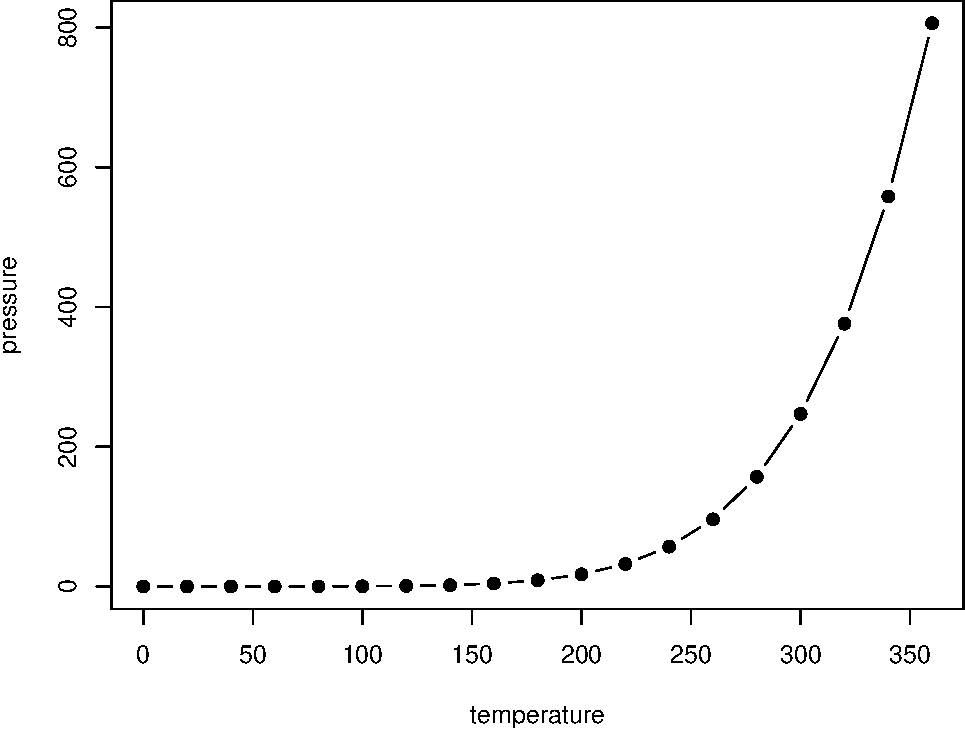
\includegraphics[width=0.8\linewidth]{10-Test_files/figure-latex/nice-fig-1} 

}

\caption{Here is a nice figure!}\label{fig:nice-fig}
\end{figure}

And an external figure \ref{fig:test}

\begin{figure}

{\centering 
\includegraphics[width=0.45\linewidth]{cover/pictures/back-bg} 

}

\caption{Example pic}\label{fig:test}
\end{figure}

\bibliography{bib/thesis.bib}

\end{document}
